
\begin{frame}[fragile]{Construction d'une requête SQL}


\begin{redbullet}
  \item Le \emph{résultat} d'une requête est une relation constituée de nuplets.
  \item  Chaque nuplet du résultat est construit à partir d'un ensemble de $n$  nuplets 
       $t_1, t_2, \cdots, t_n$  \emph{provenant de la base de données}.  
       \item Ces  $n$ nuplets  doivent satisfaire un ensemble de \emph{conditions} (exprimé par une formule)
\end{redbullet}

\vfill

La clause \sqlkw{from} sert à définir les $t_1, t_2, \cdots, t_n$, la clause \sqlkw{where}
à définir les conditions, la clause \sqlkw{select} à construire un nuplet-résultat 
à partir des $t_1, t_2, \cdots, t_n$.

\vfill
Dans cette session nous étudions le processus (mental) de conception d'une requête.

\vfill
\begin{blocgauche}
\alert{Ces diapositives correspondent au support en ligne disponible sur
le site \url{http://sql.bdpedia.fr/}}
\end{blocgauche}

\end{frame}



\begin{frame}{Etape prélable\,: comprendre le schéma}

Il faut savoir visualiser les tables, et les liens (clé primaire, clé étrangère).
\vfill


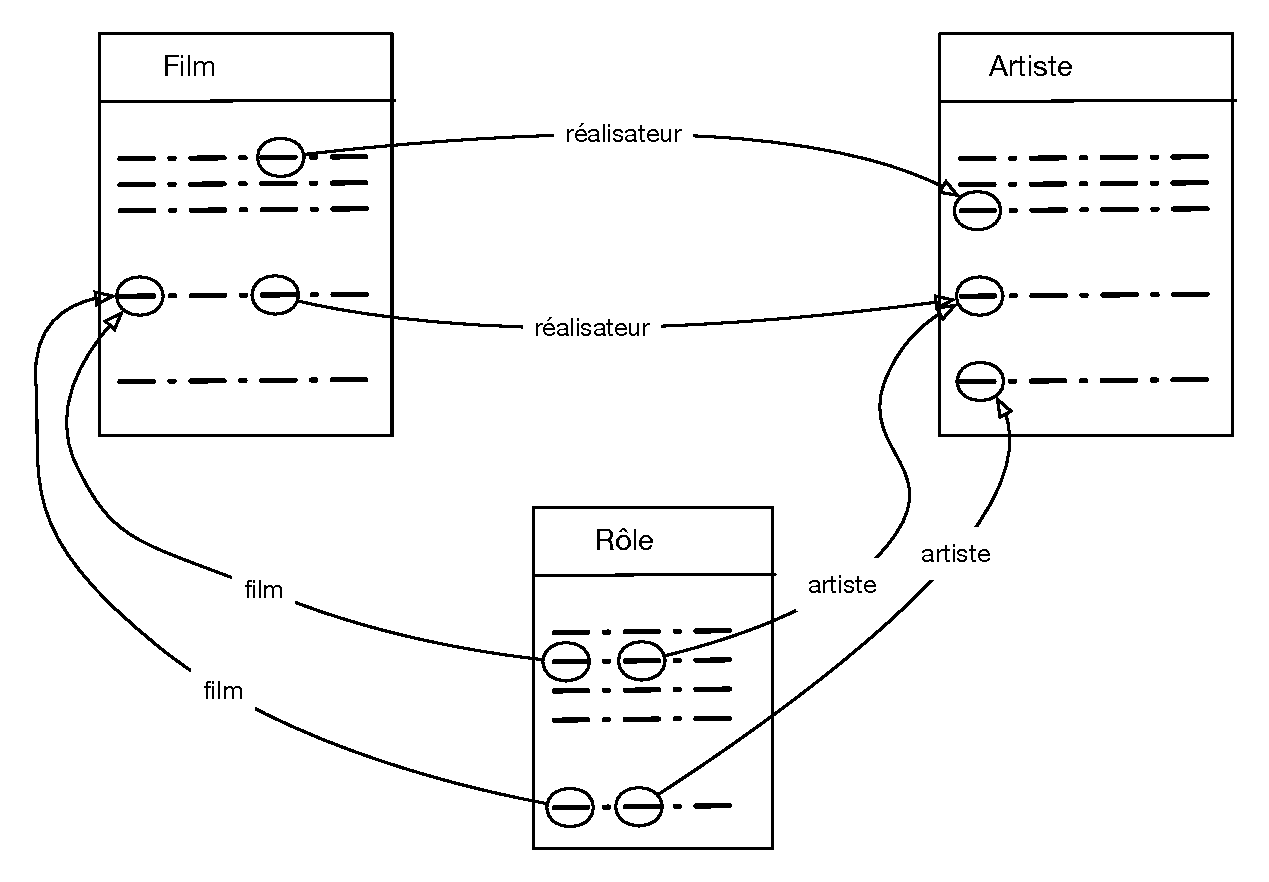
\includegraphics[width=10cm]{../figures-sql/construireSQL1}
\end{frame}


\begin{frame}[fragile]{Imaginer une requête = visualiser les nuplets}

\vspace*{0.5cm}

\begin{tabular}{p{7cm}p{6cm}}

Exemple trivial\,:

``Quel âge a Gérard Depardieu\,?''

\vfill

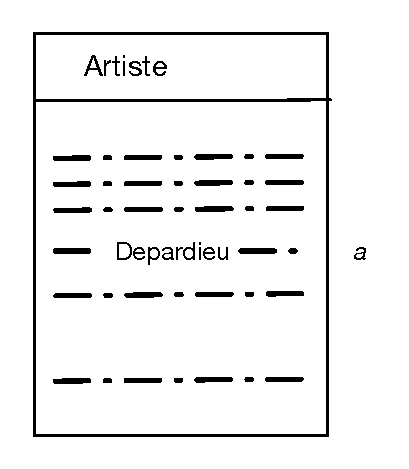
\includegraphics[width=4cm]{../figures-sql/construireSQLDepardieu}

\vfill

On identifie un nuplet, $a$, qui suffit.
&
La requête est une transcription directe de la visualisation.

\vfill

\begin{minted}[baselinestretch=.9,
               fontsize=\large,
               framesep=2mm]{sql}
    select annéeNaissance
     from Artiste as a
     where a.nom='Depardieu'
\end{minted}

\vfill

Pour l'instant tout est simple.
\end{tabular}

\end{frame}


\begin{frame}[fragile]{Souvent il faut plusieurs nuplets}


\vfill

\begin{tabular}{p{7cm}p{6cm}}


Exemple les films avec Gérard Depardieu\,?
\bigskip

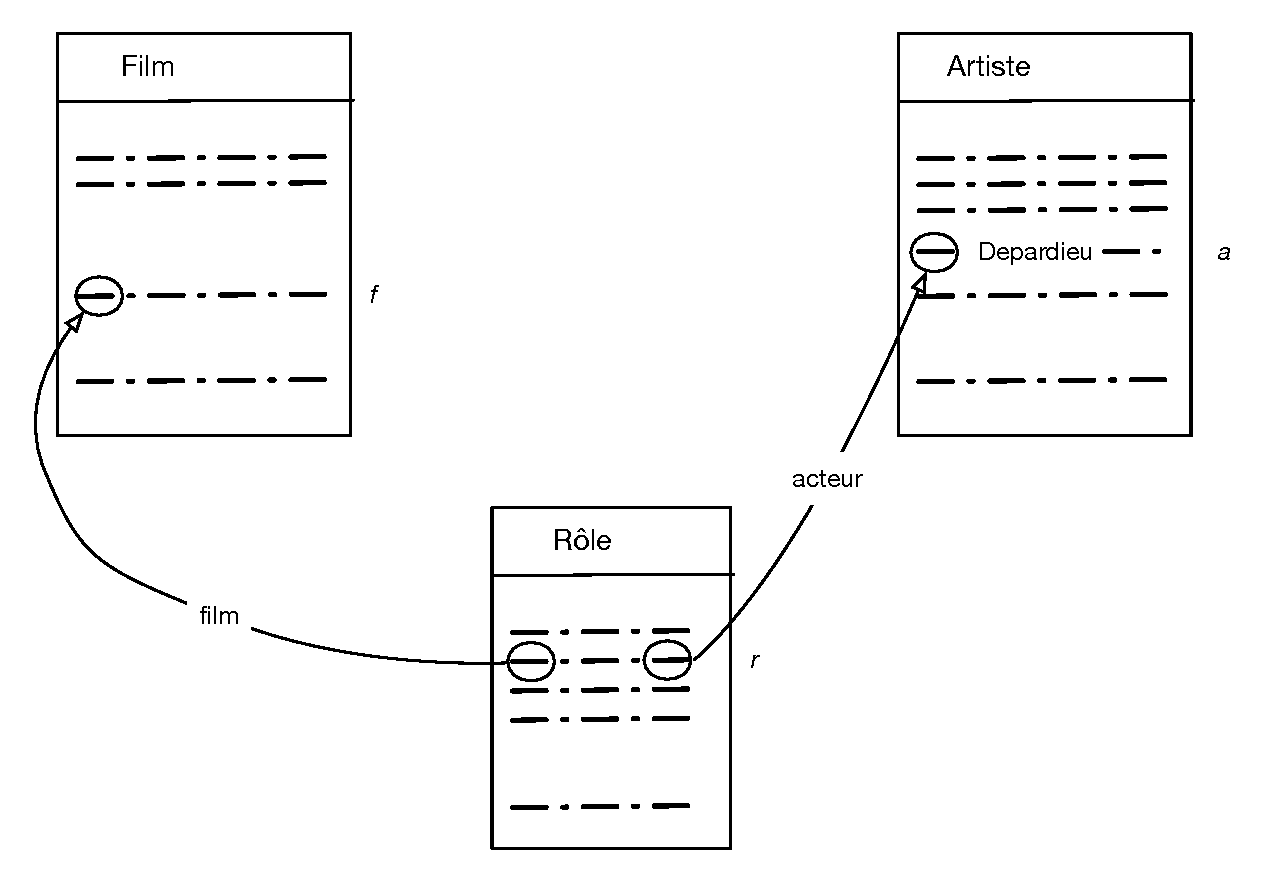
\includegraphics[width=7cm]{../figures-sql/construireSQLDepardieuFilm}

&

\begin{minted}[baselinestretch=.9,
               fontsize=\small,
               framesep=2mm]{sql}
select f.titre
from Artiste as a, Rôle as r, Film as f
where a.nom='Depardieu'
and a.idArtiste = r.idActeur
and r.idFilm = f.idFilm
\end{minted}

\vfill

La requête est encore une transcription directe de la visualisation.
\end{tabular}

\end{frame}



\begin{frame}[fragile]{Les films avec C. Deneuve et G. Depardieu}


\vfill

\begin{tabular}{p{8cm}p{5cm}}

\bigskip

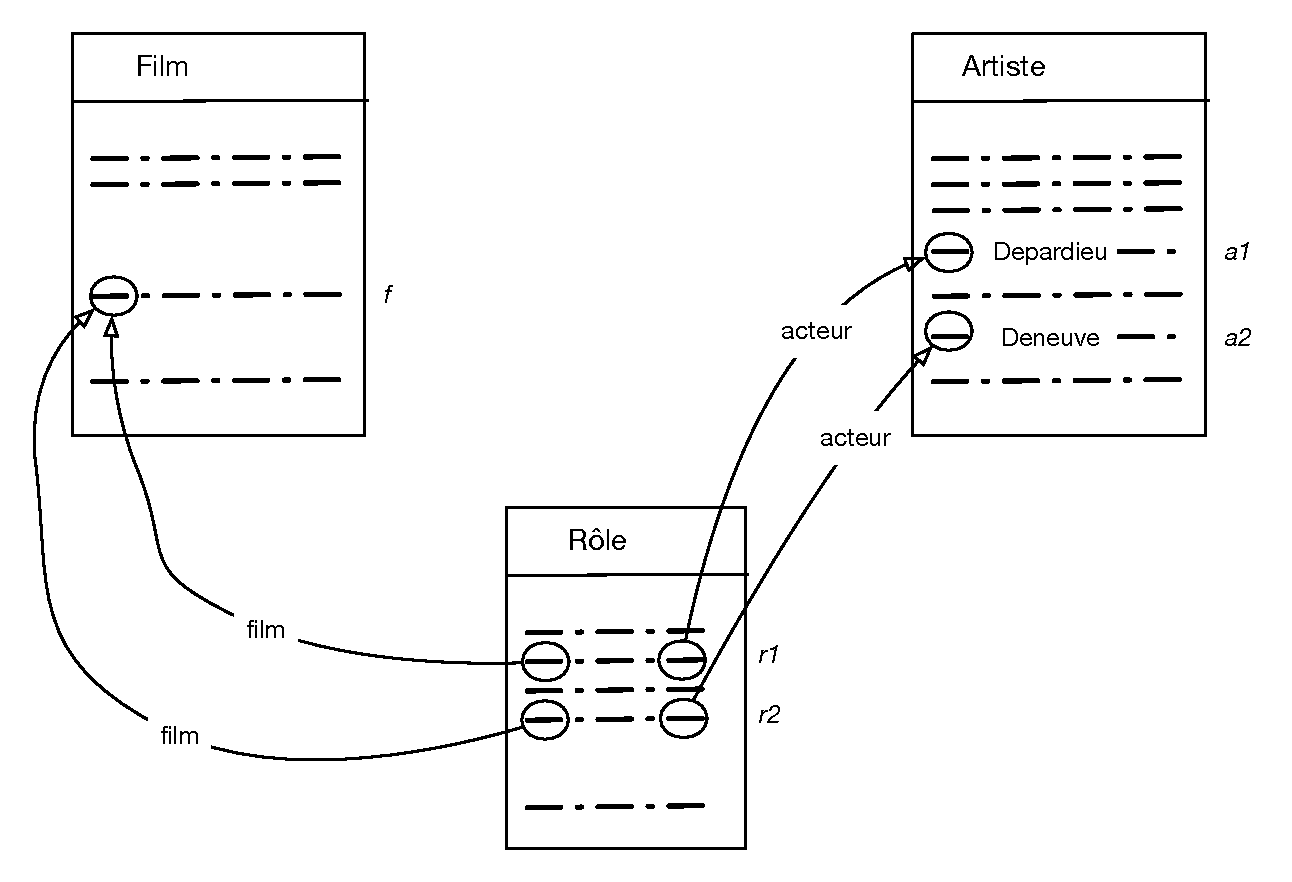
\includegraphics[width=8cm]{../figures-sql/construireSQLDepardieuDeneuveFilm}

&


\begin{minted}[baselinestretch=.9,
               fontsize=\small,
               framesep=2mm]{sql}
select * 
from Artiste as a1, Artiste as a2, 
     Rôle as r1,  Rôle as r2, 
     Film as f
where a1.nom='Depardieu'
and a2.nom='Deneuve'
and a1.idArtiste = r1.idActeur
and a2.idArtiste = r2.idActeur
and r1.idFilm = f.idFilm
and r2.idFilm = f.idFilm
\end{minted}

\end{tabular}

\end{frame}


\begin{frame}[fragile]{Les films réalisés par Q. Tarantino en 1994}


\vfill

\begin{tabular}{p{8cm}p{5cm}}

\bigskip
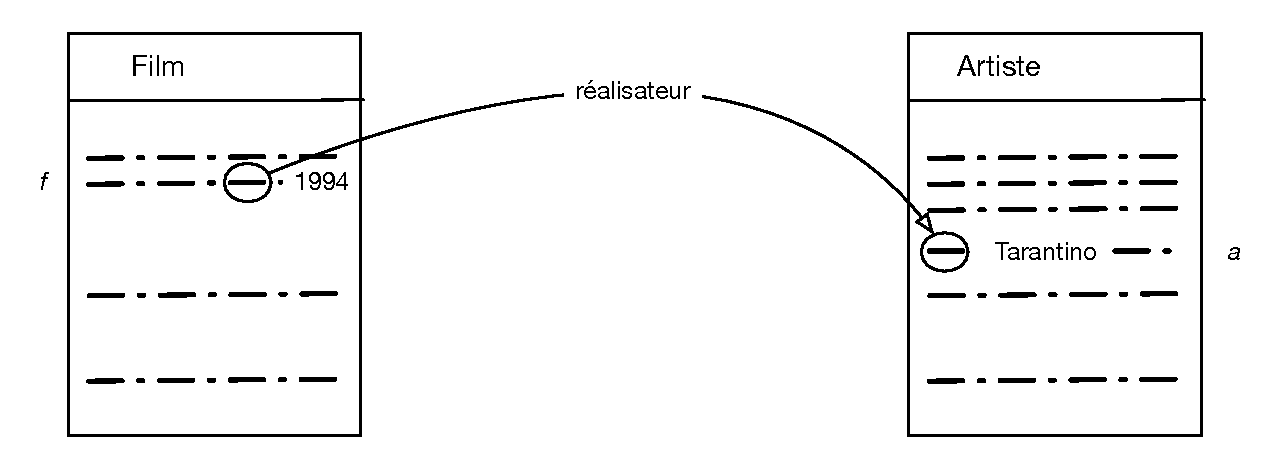
\includegraphics[width=8cm]{../figures-sql/construireSQLTarantinoFilm}

&


\begin{minted}[baselinestretch=.9,
               fontsize=\small,
               framesep=2mm]{sql}
select * 
from Artiste as a, Film as f
where a.nom='Tarantino'
and  f.année = 1994
and a.idArtiste = f.idRéalisateur
\end{minted}

\end{tabular}
\end{frame}


\begin{frame}[fragile]{Les films réalisés par Q. Tarantino en 1994 dans lesquels il joue}



\vfill

\begin{tabular}{p{8cm}p{5cm}}

\bigskip
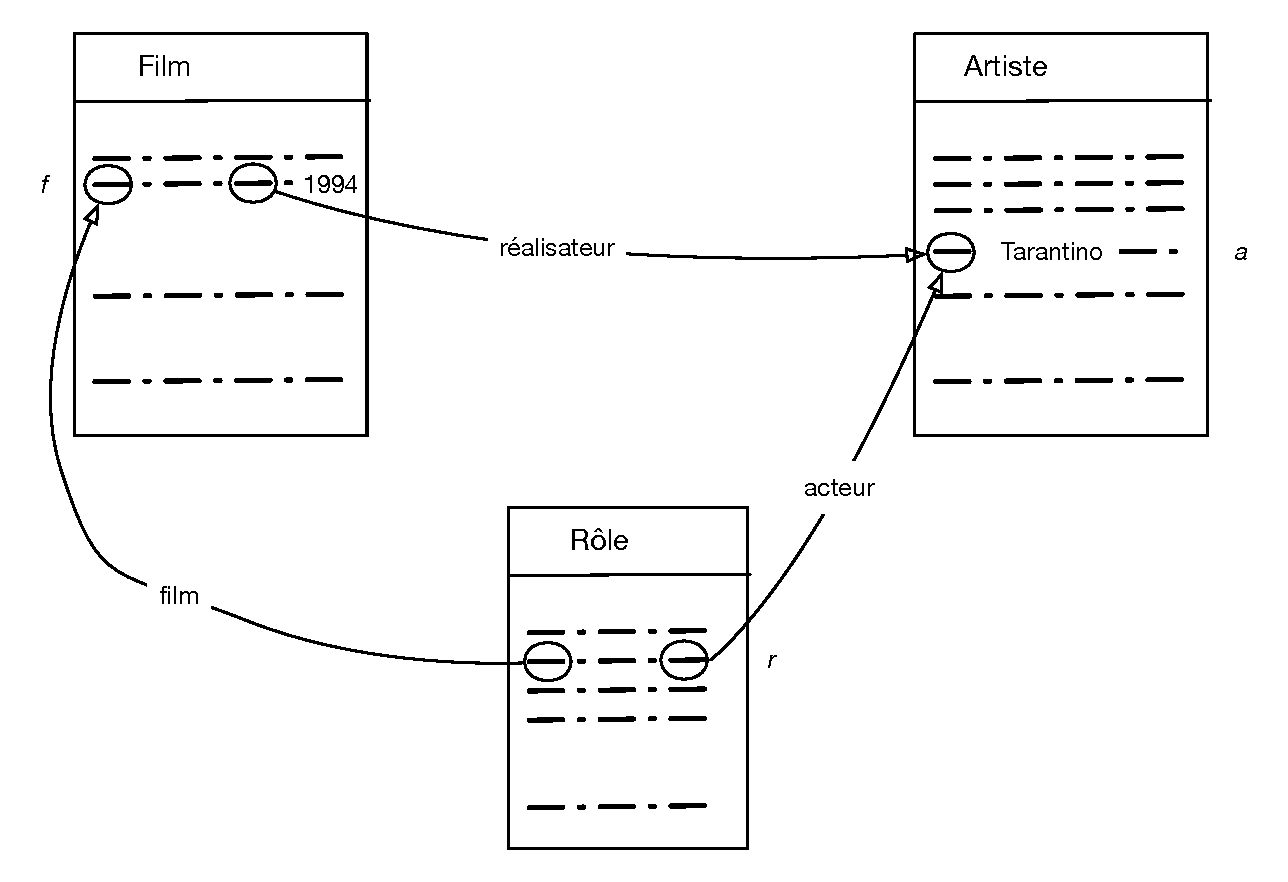
\includegraphics[width=8cm]{../figures-sql/construireSQLTarantinoFilmArtiste}

&

\bigskip

Requête\,: à vous de jouer!

\end{tabular}
\end{frame}



%%%%%%%%%
\begin{frame}{À retenir}

\vfill

La démarche mentale pour construire une requête SQL est (toujours) la suivante

\vfill

\begin{redbullet}
  \item  \alert{On détermine les nuplets (et leur table)} nécessaires pour construire
     un nuplet du résultat
     
        $\Rightarrow$ ça définit le \sqlkw{from}

  \item \alert{On détermine les conditions que doivent satisfaire ces nuplets }
  
        $\Rightarrow$ ça définit le \sqlkw{where}
    \smallskip
    
    \alert{Important}\,: une condition peut être définie par une sous-requête (résultat vide ou non)
    
   \item  \alert{Il ne reste plus qu'à ``piocher'' dans les nuplets pour constituer le résultat }
   
           $\Rightarrow$ ça définit le \sqlkw{select} et la requête complète.
   
\end{redbullet}

\vspace*{1cm}

\end{frame}



